\documentclass[10pt]{article}
\usepackage{tikz}
\usetikzlibrary{shapes.misc}
\usepackage[margin=0cm]{geometry}
\pagestyle{empty}
\tikzstyle{every node}=[cross out, draw, red]

\begin{document}

\vspace*{\fill}
\begin{center}
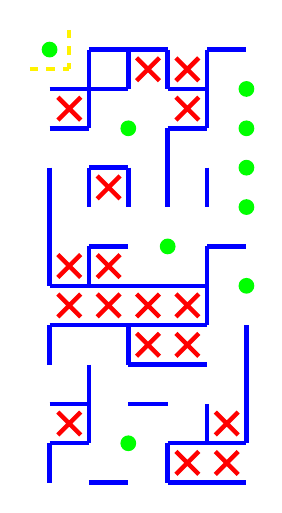
\begin{tikzpicture}[x=0.5cm, y=-0.5cm, ultra thick, blue]
% Walls
    \draw (1,0) -- (3,0);
    \draw (4,0) -- (5,0);
    \draw (0,1) -- (2,1);
    \draw (3,1) -- (4,1);
    \draw (0,2) -- (1,2);
    \draw (3,2) -- (4,2);
    \draw (1,3) -- (2,3);
    \draw (1,5) -- (2,5);
    \draw (4,5) -- (5,5);
    \draw (0,6) -- (4,6);
    \draw (0,7) -- (4,7);
    \draw (2,8) -- (4,8);
    \draw (0,9) -- (1,9);
    \draw (2,9) -- (3,9);
    \draw (0,10) -- (1,10);
    \draw (3,10) -- (5,10);
    \draw (1,11) -- (2,11);
    \draw (3,11) -- (5,11);
    \draw (0,3) -- (0,6);
    \draw (0,7) -- (0,8);
    \draw (0,10) -- (0,11);
    \draw (1,0) -- (1,2);
    \draw (1,3) -- (1,4);
    \draw (1,5) -- (1,6);
    \draw (1,8) -- (1,10);
    \draw (2,0) -- (2,1);
    \draw (2,3) -- (2,4);
    \draw (2,7) -- (2,8);
    \draw (3,0) -- (3,1);
    \draw (3,2) -- (3,4);
    \draw (3,10) -- (3,11);
    \draw (4,0) -- (4,2);
    \draw (4,3) -- (4,4);
    \draw (4,5) -- (4,7);
    \draw (4,9) -- (4,10);
    \draw (5,7) -- (5,10);
% Pillars
    \fill[green] (0,0) circle(0.2);
    \fill[green] (5,1) circle(0.2);
    \fill[green] (2,2) circle(0.2);
    \fill[green] (5,2) circle(0.2);
    \fill[green] (5,3) circle(0.2);
    \fill[green] (5,4) circle(0.2);
    \fill[green] (3,5) circle(0.2);
    \fill[green] (5,6) circle(0.2);
    \fill[green] (2,10) circle(0.2);
% Inner points in accessible cul-de-sacs
    \node at (2.5,0.5) {};
    \node at (3.5,0.5) {};
    \node at (0.5,1.5) {};
    \node at (3.5,1.5) {};
    \node at (1.5,3.5) {};
    \node at (0.5,5.5) {};
    \node at (1.5,5.5) {};
    \node at (0.5,6.5) {};
    \node at (1.5,6.5) {};
    \node at (2.5,6.5) {};
    \node at (3.5,6.5) {};
    \node at (2.5,7.5) {};
    \node at (3.5,7.5) {};
    \node at (0.5,9.5) {};
    \node at (4.5,9.5) {};
    \node at (3.5,10.5) {};
    \node at (4.5,10.5) {};
% Entry-exit paths without intersections
    \draw[dashed, yellow] (-0.5,0.5) -- (0.5,0.5);
    \draw[dashed, yellow] (0.5,-0.5) -- (0.5,0.5);
\end{tikzpicture}
\end{center}
\vspace*{\fill}

\end{document}
